\documentclass[slidestop,compress,mathserif,c]{beamer}
\usepackage{listings}
\usepackage{color}
\usepackage{xcolor}
\usepackage{hyperref}
\definecolor{dkgreen}{rgb}{0,0.6,0}
\usepackage{fontspec,xunicode,xltxtra,beamerthemesplit}
%\usepackage{slashbox}
\usepackage{diagbox}
 \newfontfamily\times{Times New Roman}
%以下是各种演示主题,定义幻灯片中的所有细节
%\usetheme{default}
%\usetheme{Berlin}%这个主题比较好
%\usetheme{Pittsburgh}
%\usetheme{Rochester}
\usetheme{Berkeley}%这种演示主题比较好
%\usetheme{Goettingen}
%\usetheme{Hannover}
%\usetheme{Marburg}
%\usetheme{PaloAlto}%这种演示主题比较好
%\usetheme{Antibes}
%\usetheme{Darmstadt}
%\usetheme{JuanLesPins}
%\usetheme{Montpellier}
%\usetheme{Singapore}
%\usetheme{Boadilla}
%\usetheme{Madrid}
%\usetheme{AnnArbor}
%\usetheme{CambridgeUS}
%\usetheme{Copenhagen}
%\usetheme{Warsaw}

%以下是各种外部主题,确定幻灯的显示式样
%\useoutertheme{infolines}
%\useoutertheme{miniframes}
%\useoutertheme[height=0.1\textwidth,width=0.15\textwidth,hideothersubsections]{sidebar}
%\useoutertheme{smoothbars}
%\useoutertheme{split}
%\useoutertheme{shadow}
%\useoutertheme{tree}
%\useoutertheme{smoothtree}
%\useoutertheme[height=0.5\textwidth]{sidebar}

%以下是各种内部主题
%\useinnertheme{default}
%\useinnertheme{circles}
%\useinnertheme{rectangles}
\useinnertheme[shadow]{rounded}

%以下是各种颜色主题
%\usecolortheme{default}
%\usecolortheme{albatross}
%\usecolortheme{beaver}
%\usecolortheme{beetle}
%\usecolortheme{crane}
%\usecolortheme{dolphin}
%\usecolortheme{dove}
%\usecolortheme{fly}
%\usecolortheme{lily}
%\usecolortheme{orchid}
%\usecolortheme{rose}
%\usecolortheme{seagull}
\usecolortheme{seahorse}
%\usecolortheme{sidebartab}
%\usecolortheme{structure}
%\usecolortheme{whale}
%\usecolortheme{wolverine}

%以下是各种字体主题
%\usefonttheme{default}
%\usefonttheme[onlymath]{serif}
%\usefonttheme{structurebold}
%\usefonttheme{structureitalicserif}
%\usefonttheme{structuresmallcapsserif}
\newcommand{\tablecell}[2]{\begin{tabular}{@{}#1@{}}#2\end{tabular}}   % 表格内换行,用法\tablecell{c}{balabalba\\balabalba}
\setsansfont[Mapping=tex-text, BoldFont={微软雅黑 Bold}]{微软雅黑}

% 中文环境自动换行
\XeTeXlinebreaklocale "zh"  % 表示用中文的断行
\XeTeXlinebreakskip = 0pt plus 1pt % 多一点调整的空间

% 中文环境修正导航栏
\makeatletter
\setbeamertemplate{blocks}[rounded][shadow=true] 
\def\beamer@linkspace#1{
  \begin{pgfpicture}{0pt}{-1.5pt}{#1}{5.5pt}
    \pgfsetfillopacity{0}
    \pgftext[x=0pt,y=-1.5pt]{.}
    \pgftext[x=#1,y=5.5pt]{.}
  \end{pgfpicture}}
\makeatother

% 超链接高亮显示
\hypersetup{CJKbookmarks=true,
colorlinks=true,
citecolor=blue,
linkcolor=blue,
urlcolor=blue,
bookmarksopen=true,
breaklinks=true
}

% 幻灯片切换方式
%\transblindshorizontal 	% 水平百叶窗
%\transblindsvertical 		% 垂直百叶窗
%\transboxin				% 盒状收缩
%\transboxout				% 盒状展开
%\transdissolve				% 溶解
%\transglitter
%\transsplithorizontalin	% 上下向中央收缩
%\transsplitverticalin		% 垂直向中央收缩
%\transsplithorizontalout	% 上下向中央展开
%\transsplitverticalout		% 垂直向中央展开
%\transwipe					% 从下抽出


\title{BP神经网络}
\author{Liu Zheng}
\date{\today}
\institute{同济大学电信学院}

\logo{\color{blue!50}\scalebox{2}{{
\includegraphics[height=0.8cm]{logo.jpg}\vspace{220pt}}}}

% 设定frametitle居中
\makeatletter 
\long\def\beamer@@frametitle[#1]#2{% 
  \beamer@ifempty{#2}{}{% 
    \gdef\insertframetitle{\centering{#2\ifnum\beamer@autobreakcount>0\relax{}\space\usebeamertemplate*{frametitle continuation}\fi}}% 
  \gdef\beamer@frametitle{#2}% 
  \gdef\beamer@shortframetitle{#1}% 
}% 
} 
\makeatother


\titlegraphic{
\includegraphics[width=2.3cm]{qr.png}}
\begin{document}

\frame{\titlepage}
\AtBeginSection{
  \frame{\tableofcontents[sections={\thesection}]}
}
\section{BP神经网络概述}


%%%%%%%%%% One Slide %%%%%%%%%%
%\subsection{Overview}
\begin{frame}
\frametitle{BP神经网络概述}
~~~~~~神经网络是单个并行处理元素的集合,我们从生物学神经系统得到启发。在自然界,网络功能主要由神经节决定,我们可以通过改变连接点的权重来训练神经网络完成特定的功能。

~~~~~~一般的神经网络都是可调节的,或者说可训练的,这样一个特定的输入便可得到要求的输出。如下图所示。这里,网络根据输出和目标的比较而调整,直到网络输出和目标匹配。作为典型,许多输入/目标对应的方法已被用在有监督模式中来训练神经网络。 

\end{frame}
%%%%%%%%%% Slide End %%%%%%%%%%

%%%%%%%%%% One Slide %%%%%%%%%%
%\subsection{Overview}
\begin{frame}
\frametitle{Overview}
~~~~~~一种常见的多层结构的前馈网络(Multilayer Feedforward Network)由三部分组成

\begin{itemize}
\item 输入层(Input layer),众多神经元(Neuron)接受大量非线形输入信息。输入的信息称为输入向量。
\item 输出层(Output layer),信息在神经元链接中传输、分析、权衡,形成输出结果。输出的信息称为输出向量。
\item 隐藏层(Hidden layer),简称“隐层”,是输入层和输出层之间众多神经元和链接组成的各个层面。隐层可以有多层,习惯上会用一层。隐层的节点(神经元)数目不定,但数目越多神经网络的非线性越显著,从而神经网络的强健性(robustness)(控制系统在一定结构、大小等的参数摄动下,维持某些性能的特性。)更显著。习惯上会选输入节点1.2至1.5倍的节点。
\end{itemize}
\end{frame}
%%%%%%%%%% Slide End %%%%%%%%%%


%%%%%%%%%% One Slide %%%%%%%%%%
\subsection{神经对比}
\begin{frame}
\frametitle{神经对比}
\begin{figure}
\centering
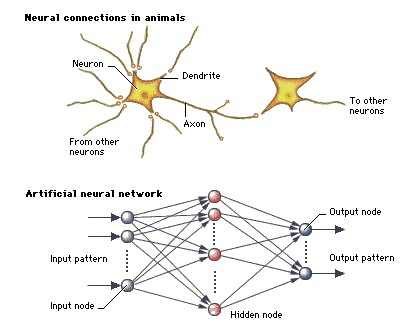
\includegraphics[width=8cm]{img1}
\end{figure}
\end{frame}
%%%%%%%%%% Slide End %%%%%%%%%%


%%%%%%%%%% One Slide %%%%%%%%%%
\subsection{神经元示意图}
\begin{frame}
\frametitle{神经元示意图}
\begin{figure}
\centering
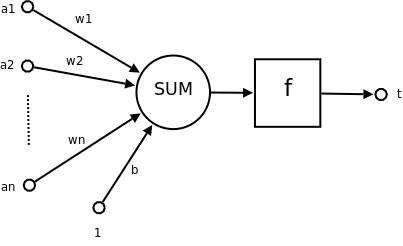
\includegraphics[width=7cm]{Ncell}
\end{figure}~\\[-1.1cm]
$a_1\sim a_n$ 为输入向量的各个分量

$w_1\sim w_n$ 为神经元各个突触的权值

$b$ 为偏置~~~~、~~~~$t$ 为神经元输出

$f$ 为传递函数,通常为非线性函数。一般有traingd(), tansig(), hardlim()。一般为hardlim()


\end{frame}
%%%%%%%%%% Slide End %%%%%%%%%%


%%%%%%%%%% One Slide %%%%%%%%%%
%\subsection{Overview}
\begin{frame}
\frametitle{数学表示}
\resizebox{\textwidth}{!}{$t = f(\vec{W}\vec{A'}+b)$}
~\\[1cm]
$ \vec{W} $ 为权向量

$ \vec{A} $为输入向量,$\vec{A'} $ 为$\vec{A}$的转置

$b$ 为偏置

$f$ 为传递函数
\end{frame}
%%%%%%%%%% Slide End %%%%%%%%%%
\section{传递函数}
%%%%%%%%%% One Slide %%%%%%%%%%
\subsection{输入,输出层的激励函数}
\begin{frame}
\frametitle{tansig}
\begin{figure}
\centering
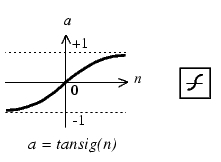
\includegraphics[width=7cm]{tansig_TFMATLAB}
\end{figure}
%输入,输出层的激励函数

\end{frame}
%%%%%%%%%% Slide End %%%%%%%%%%

%%%%%%%%%% One Slide %%%%%%%%%%
%\subsection{传递函数}
\begin{frame}
\frametitle{purelin}
\begin{figure}
\centering
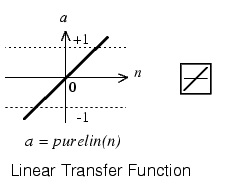
\includegraphics[width=7cm]{purelin}
\end{figure}
%输入,输出层的激励函数
\end{frame}
%%%%%%%%%% Slide End %%%%%%%%%%


%%%%%%%%%% One Slide %%%%%%%%%%
%\subsection{传递函数}
\begin{frame}
\frametitle{hardlim}
\begin{figure}
\centering
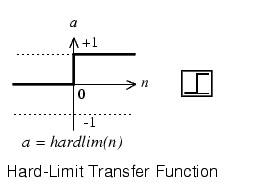
\includegraphics[width=7cm]{hardlim}
\end{figure}

%输入,输出层的激励函数

\end{frame}
%%%%%%%%%% Slide End %%%%%%%%%%



%%%%%%%%%% One Slide %%%%%%%%%%
%\subsection{传递函数}
\begin{frame}
\frametitle{logsig}
\begin{figure}
\centering
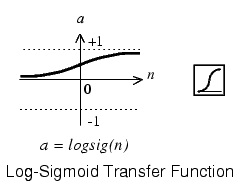
\includegraphics[width=7cm]{logsig}
\end{figure}

%输入,输出层的激励函数
\end{frame}
%%%%%%%%%% Slide End %%%%%%%%%%

%\section{学习函数}
%%%%%%%%%% One Slide %%%%%%%%%%
\subsection{学习函数}
\begin{frame}
\frametitle{learngd}
~~~~~~函数learngd有一个相关的参数--学习速率lr。权重和偏置的变化通过梯度的负数乘上学习速率倍数得到。学习速率越大,步进越大。如果学习速率太大算法就会变得不稳定。如果学习速率太小,算法就需要很长的时间才能收敛。当learnFcn设置为learngd时,就为每一个权重和偏置设置了学习速率参数的缺省值。

\end{frame}
%%%%%%%%%% Slide End %%%%%%%%%%


%%%%%%%%%% One Slide %%%%%%%%%%
%\subsection{Overview}
\begin{frame}
\frametitle{leardgdm(带动力的梯度下降法)}
~~~~~~除了learngd以外,还有一种增加方式算法常被用到,它能提供更快的收敛速度--learngdm,带动量的最速下降法。动力允许网络不但根据当前梯度而且还能根据误差曲面最近的趋势响应。就像一个低通滤波器一样,动量允许网络忽略误差曲面的小特性。没有动量,网络又可能在一个局部最小中被卡住。有了动量网络就能够平滑这样的最小。动量能够通过把权重变得与上次权重变化的部分和由算法规则得到的新变化的和相同而加入到网络学习中去。上一次权重变化对动量的影响由一个动量常数来决定,它能够设为0到1之间的任意值。当动量常数为0时,权重变化之根据梯度得到。当动量常数为1时新的权重变化等于上次的权重变化,梯度值被忽略了。

\end{frame}
%%%%%%%%%% Slide End %%%%%%%%%%


%%%%%%%%%% One Slide %%%%%%%%%%
%\subsection{Overview}
\begin{frame}
\frametitle{Overview}


\end{frame}
%%%%%%%%%% Slide End %%%%%%%%%%


%%%%%%%%%% One Slide %%%%%%%%%%
%\subsection{Overview}
\begin{frame}
\frametitle{Overview}


\end{frame}
%%%%%%%%%% Slide End %%%%%%%%%%

\section{MATLAB演示}
%%%%%%%%%% One Slide %%%%%%%%%%
%\subsection{}
\begin{frame}
\frametitle{Neural Network GUI}
Open the Neural Network Start GUI with this command:
nnstart
\begin{figure}
\centering
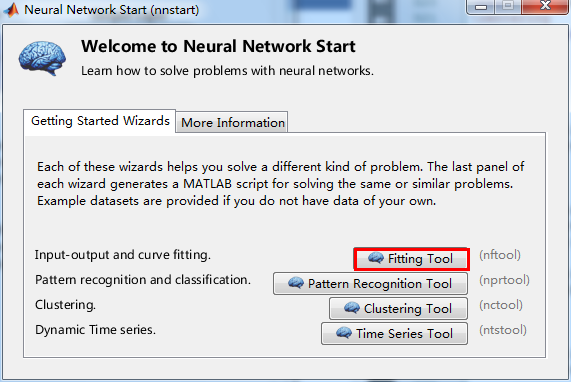
\includegraphics[width=7cm]{1}
\end{figure}


\end{frame}
%%%%%%%%%% Slide End %%%%%%%%%%


%%%%%%%%%% One Slide %%%%%%%%%%
%\subsection{}
\begin{frame}
\frametitle{Neural Network GUI}

\begin{figure}
\centering
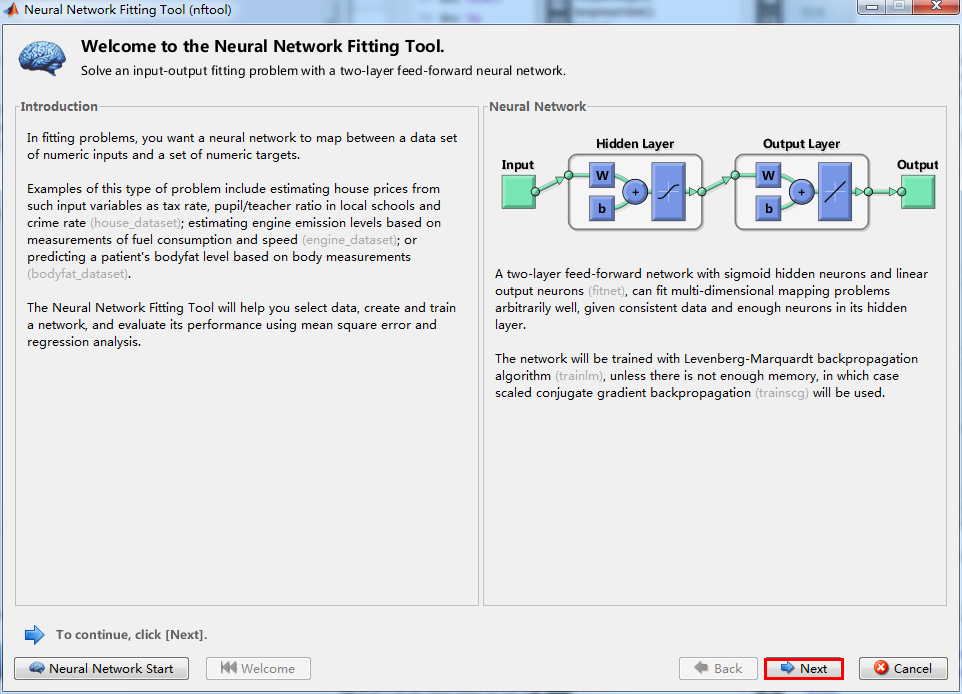
\includegraphics[width=8cm]{2}
\end{figure}


\end{frame}
%%%%%%%%%% Slide End %%%%%%%%%%


%%%%%%%%%% One Slide %%%%%%%%%%
%\subsection{}
\begin{frame}
\frametitle{Neural Network GUI}
选择demo数据
\begin{figure}
\centering
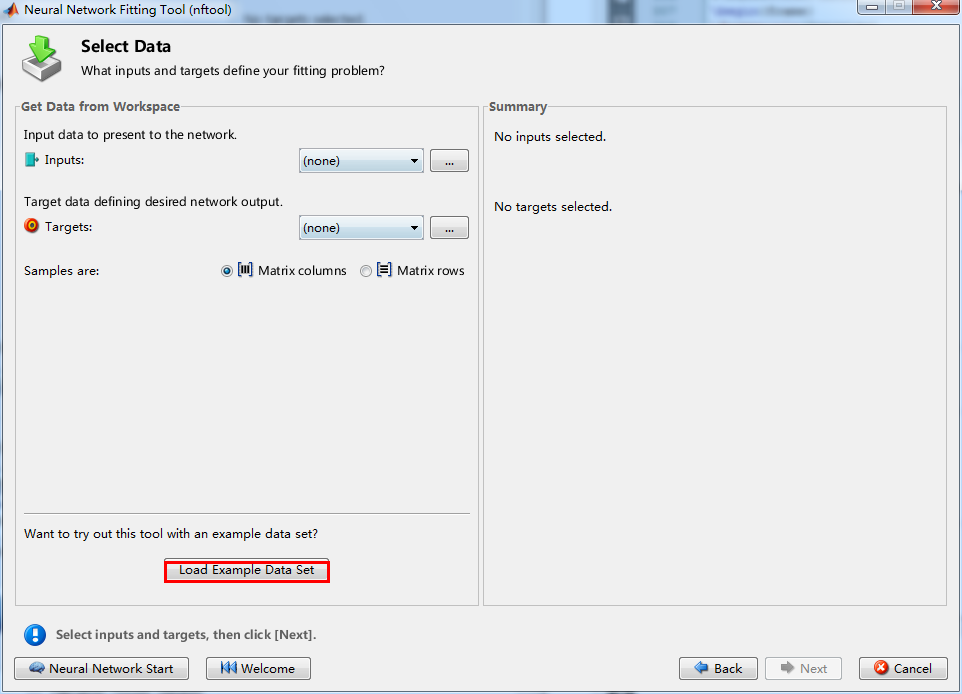
\includegraphics[width=8cm]{3}
\end{figure}


\end{frame}
%%%%%%%%%% Slide End %%%%%%%%%%


%%%%%%%%%% One Slide %%%%%%%%%%
%\subsection{}
\begin{frame}
\frametitle{Neural Network GUI}

\begin{figure}
\centering
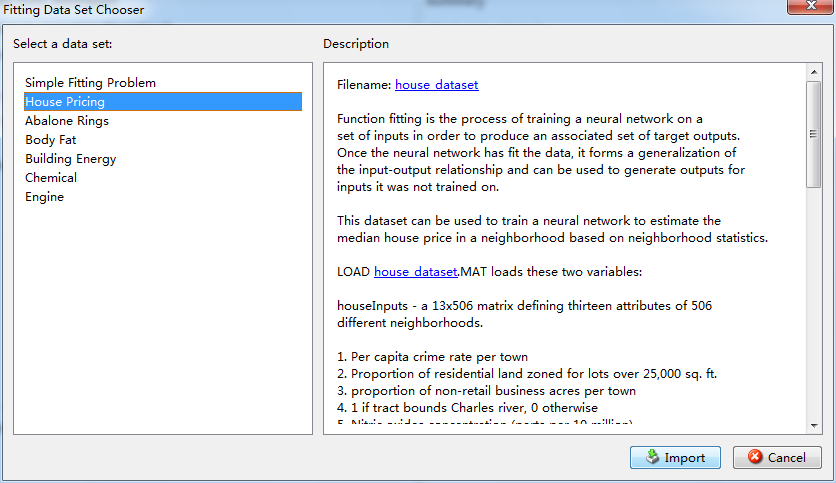
\includegraphics[width=8cm]{4}
\end{figure}


\end{frame}
%%%%%%%%%% Slide End %%%%%%%%%%


%%%%%%%%%% One Slide %%%%%%%%%%
%\subsection{}
\begin{frame}
\frametitle{Neural Network GUI}
这里可以调整训练集,验证集,测试集数据大小
\begin{figure}
\centering
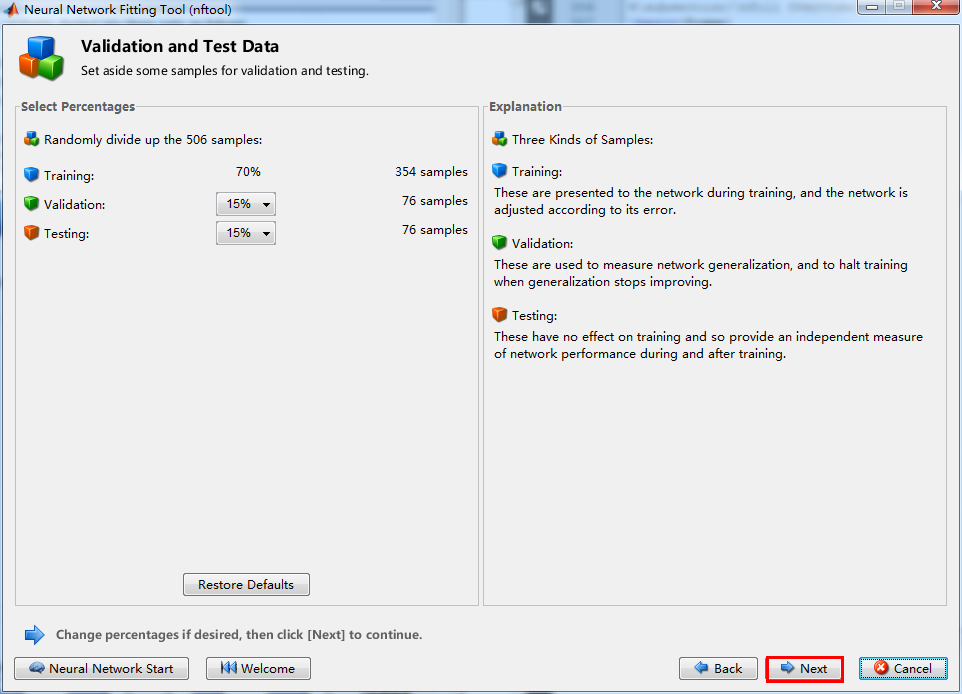
\includegraphics[width=7cm]{5}
\end{figure}


\end{frame}
%%%%%%%%%% Slide End %%%%%%%%%%

%%%%%%%%%% One Slide %%%%%%%%%%
%\subsection{}
\begin{frame}
\frametitle{Neural Network GUI}
这里可以隐层神经元的个数
\begin{figure}
\centering
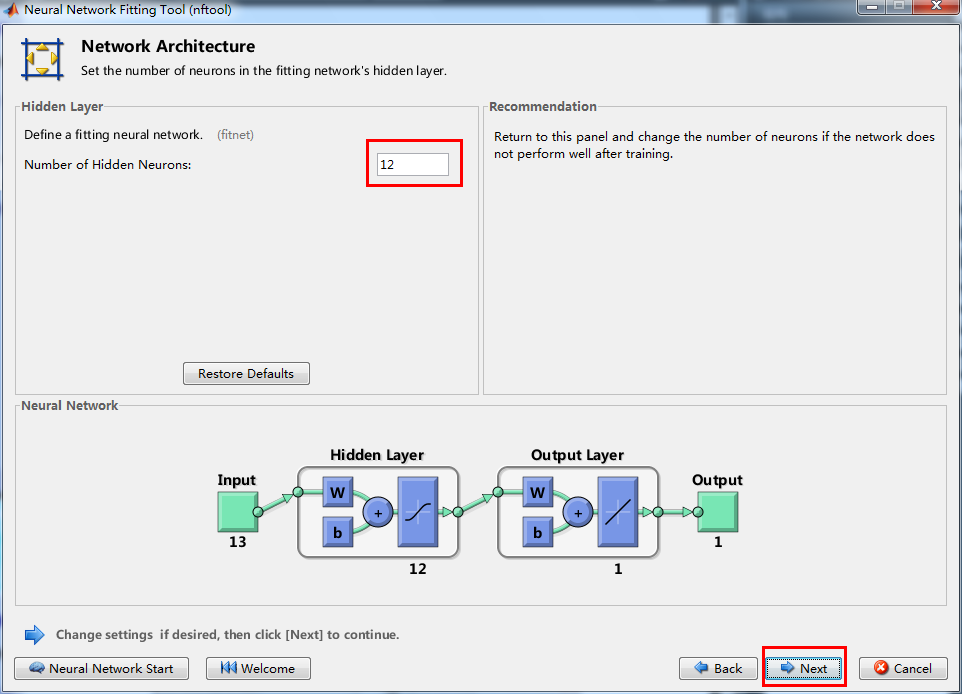
\includegraphics[width=7cm]{10}
\end{figure}


\end{frame}
%%%%%%%%%% Slide End %%%%%%%%%%


%%%%%%%%%% One Slide %%%%%%%%%%
%\subsection{}
\begin{frame}
\frametitle{Neural Network GUI}
开始训练
\begin{figure}
\centering
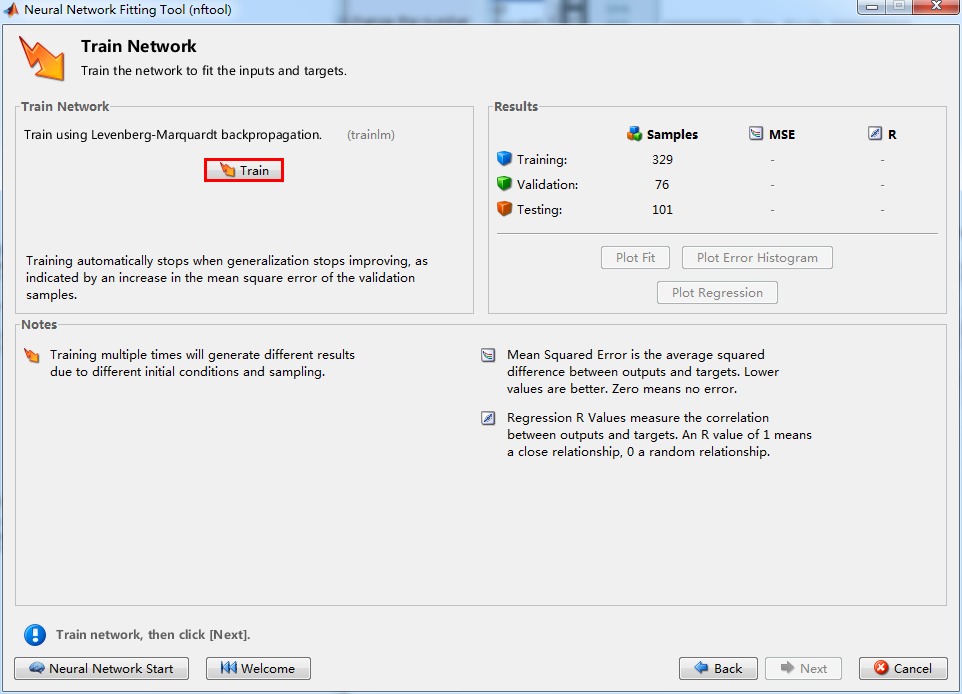
\includegraphics[width=8cm]{6}
\end{figure}


\end{frame}
%%%%%%%%%% Slide End %%%%%%%%%%


%%%%%%%%%% One Slide %%%%%%%%%%
%\subsection{}
\begin{frame}
\frametitle{Neural Network GUI}
~\\[-2.6cm]
\begin{figure}
\centering
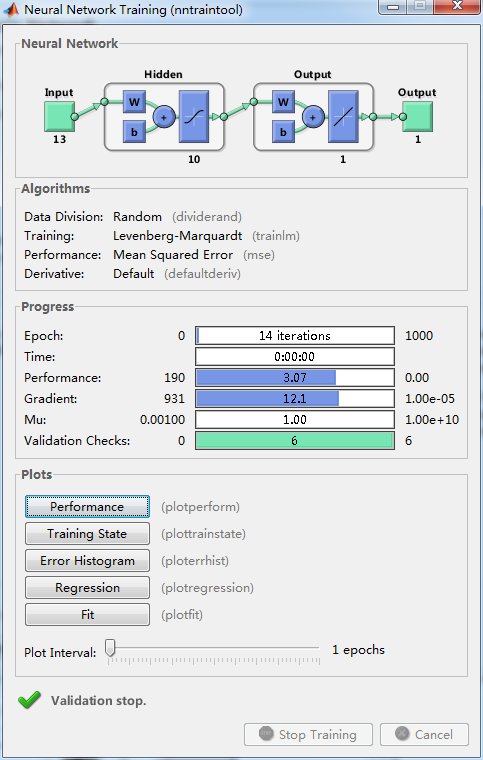
\includegraphics[width=6cm]{9}
\end{figure}


\end{frame}
%%%%%%%%%% Slide End %%%%%%%%%%


%%%%%%%%%% One Slide %%%%%%%%%%
%\subsection{}
\begin{frame}
\frametitle{Neural Network GUI}

\begin{figure}
\centering
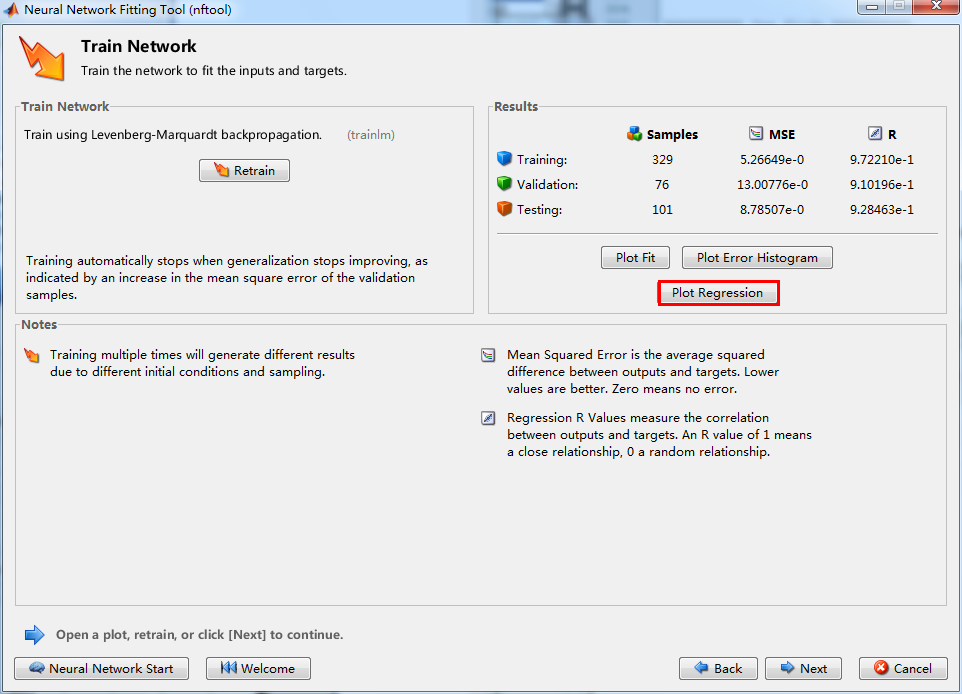
\includegraphics[width=8cm]{8}
\end{figure}


\end{frame}
%%%%%%%%%% Slide End %%%%%%%%%%

%%%%%%%%%% One Slide %%%%%%%%%%
%\subsection{}
\begin{frame}
\frametitle{Neural Network GUI}

\begin{figure}
\centering
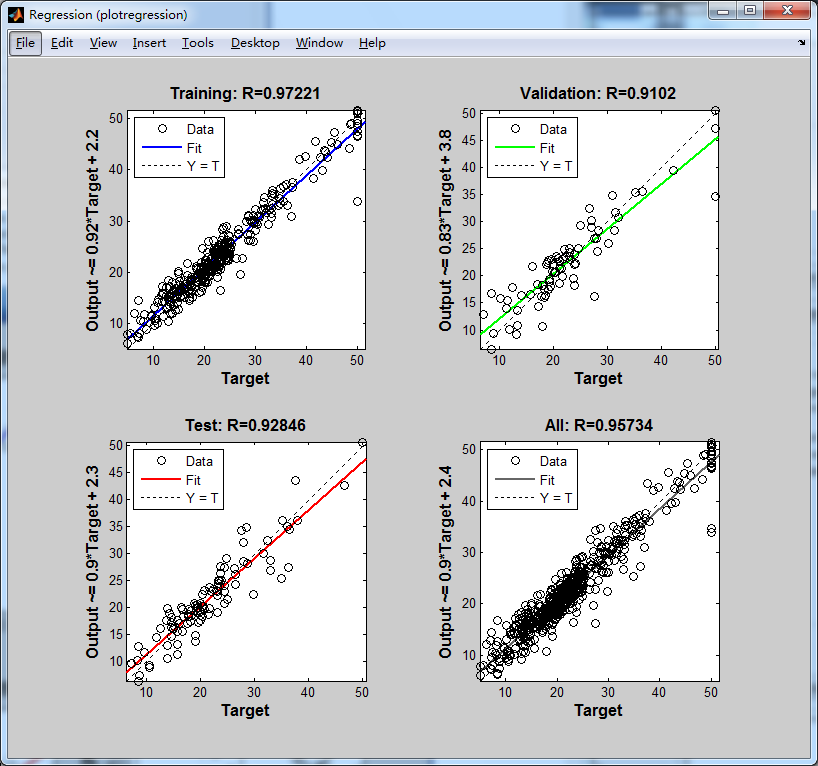
\includegraphics[width=8cm]{7}
\end{figure}
\end{frame}
%%%%%%%%%% Slide End %%%%%%%%%%

%%%%%%%%%% One Slide %%%%%%%%%%
%\subsection{}
\begin{frame}
\frametitle{Neural Network GUI}

\begin{figure}
\centering
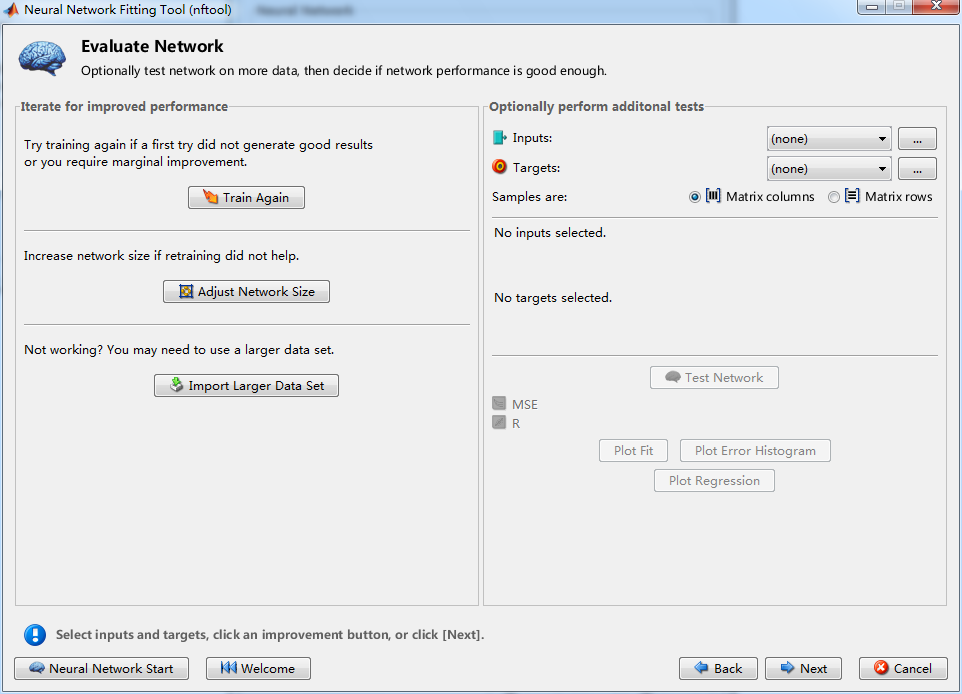
\includegraphics[width=8cm]{11}
\end{figure}
\end{frame}
%%%%%%%%%% Slide End %%%%%%%%%%

%%%%%%%%%% One Slide %%%%%%%%%%
%\subsection{}
\begin{frame}
\frametitle{Neural Network GUI}

\begin{figure}
\centering
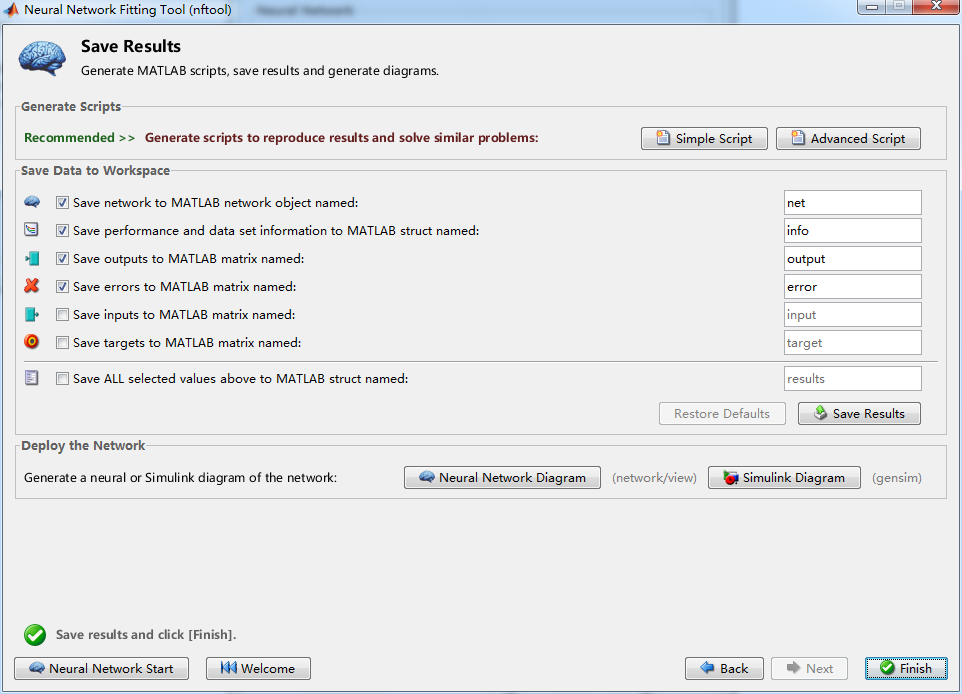
\includegraphics[width=8cm]{12}
\end{figure}
\end{frame}
%%%%%%%%%% Slide End %%%%%%%%%%


%%%%%%%%%% One Slide %%%%%%%%%%
%\subsection{Overview}
\begin{frame}
\frametitle{Overview}


\end{frame}
%%%%%%%%%% Slide End %%%%%%%%%%


\end{document}
